\documentclass[twoside]{book}

% Packages required by doxygen
\usepackage{fixltx2e}
\usepackage{calc}
\usepackage{doxygen}
\usepackage[export]{adjustbox} % also loads graphicx
\usepackage{graphicx}
\usepackage[utf8]{inputenc}
\usepackage{makeidx}
\usepackage{multicol}
\usepackage{multirow}
\PassOptionsToPackage{warn}{textcomp}
\usepackage{textcomp}
\usepackage[nointegrals]{wasysym}
\usepackage[table]{xcolor}

% Font selection
\usepackage[T1]{fontenc}
\usepackage[scaled=.90]{helvet}
\usepackage{courier}
\usepackage{amssymb}
\usepackage{sectsty}
\renewcommand{\familydefault}{\sfdefault}
\allsectionsfont{%
  \fontseries{bc}\selectfont%
  \color{darkgray}%
}
\renewcommand{\DoxyLabelFont}{%
  \fontseries{bc}\selectfont%
  \color{darkgray}%
}
\newcommand{\+}{\discretionary{\mbox{\scriptsize$\hookleftarrow$}}{}{}}

% Page & text layout
\usepackage{geometry}
\geometry{%
  a4paper,%
  top=2.5cm,%
  bottom=2.5cm,%
  left=2.5cm,%
  right=2.5cm%
}
\tolerance=750
\hfuzz=15pt
\hbadness=750
\setlength{\emergencystretch}{15pt}
\setlength{\parindent}{0cm}
\setlength{\parskip}{3ex plus 2ex minus 2ex}
\makeatletter
\renewcommand{\paragraph}{%
  \@startsection{paragraph}{4}{0ex}{-1.0ex}{1.0ex}{%
    \normalfont\normalsize\bfseries\SS@parafont%
  }%
}
\renewcommand{\subparagraph}{%
  \@startsection{subparagraph}{5}{0ex}{-1.0ex}{1.0ex}{%
    \normalfont\normalsize\bfseries\SS@subparafont%
  }%
}
\makeatother

% Headers & footers
\usepackage{fancyhdr}
\pagestyle{fancyplain}
\fancyhead[LE]{\fancyplain{}{\bfseries\thepage}}
\fancyhead[CE]{\fancyplain{}{}}
\fancyhead[RE]{\fancyplain{}{\bfseries\leftmark}}
\fancyhead[LO]{\fancyplain{}{\bfseries\rightmark}}
\fancyhead[CO]{\fancyplain{}{}}
\fancyhead[RO]{\fancyplain{}{\bfseries\thepage}}
\fancyfoot[LE]{\fancyplain{}{}}
\fancyfoot[CE]{\fancyplain{}{}}
\fancyfoot[RE]{\fancyplain{}{\bfseries\scriptsize Generated by Doxygen }}
\fancyfoot[LO]{\fancyplain{}{\bfseries\scriptsize Generated by Doxygen }}
\fancyfoot[CO]{\fancyplain{}{}}
\fancyfoot[RO]{\fancyplain{}{}}
\renewcommand{\footrulewidth}{0.4pt}
\renewcommand{\chaptermark}[1]{%
  \markboth{#1}{}%
}
\renewcommand{\sectionmark}[1]{%
  \markright{\thesection\ #1}%
}

% Indices & bibliography
\usepackage{natbib}
\usepackage[titles]{tocloft}
\setcounter{tocdepth}{3}
\setcounter{secnumdepth}{5}
\makeindex

% Custom commands
\newcommand{\clearemptydoublepage}{%
  \newpage{\pagestyle{empty}\cleardoublepage}%
}

\usepackage{caption}
\captionsetup{labelsep=space,justification=centering,font={bf},singlelinecheck=off,skip=4pt,position=top}

%===== C O N T E N T S =====

\begin{document}

% Titlepage & ToC
\pagenumbering{alph}
\begin{titlepage}
\vspace*{7cm}
\begin{center}%
{\Large Polymorphism \\[1ex]\large 4 }\\
\vspace*{1cm}
{\large Generated by Doxygen 1.8.13}\\
\end{center}
\end{titlepage}
\clearemptydoublepage
\pagenumbering{roman}
\tableofcontents
\clearemptydoublepage
\pagenumbering{arabic}

%--- Begin generated contents ---
\chapter{Hierarchical Index}
\section{Class Hierarchy}
This inheritance list is sorted roughly, but not completely, alphabetically\+:\begin{DoxyCompactList}
\item \contentsline{section}{Cell}{\pageref{classCell}}{}
\item \contentsline{section}{Grid}{\pageref{classGrid}}{}
\item \contentsline{section}{Organism}{\pageref{classOrganism}}{}
\begin{DoxyCompactList}
\item \contentsline{section}{Ant}{\pageref{classAnt}}{}
\item \contentsline{section}{Doodlebug}{\pageref{classDoodlebug}}{}
\end{DoxyCompactList}
\item \contentsline{section}{Production}{\pageref{classProduction}}{}
\item \contentsline{section}{Tests2}{\pageref{classTests2}}{}
\end{DoxyCompactList}

\chapter{Data Structure Index}
\section{Data Structures}
Here are the data structures with brief descriptions\+:\begin{DoxyCompactList}
\item\contentsline{section}{\textbf{ Ant} }{\pageref{classAnt}}{}
\item\contentsline{section}{\textbf{ Cell} }{\pageref{classCell}}{}
\item\contentsline{section}{\textbf{ Doodlebug} }{\pageref{classDoodlebug}}{}
\item\contentsline{section}{\textbf{ Grid} }{\pageref{classGrid}}{}
\item\contentsline{section}{\textbf{ Organism} }{\pageref{classOrganism}}{}
\item\contentsline{section}{\textbf{ Production} }{\pageref{classProduction}}{}
\item\contentsline{section}{\textbf{ Tests2} }{\pageref{classTests2}}{}
\end{DoxyCompactList}

\chapter{File Index}
\section{File List}
Here is a list of all files with brief descriptions\+:\begin{DoxyCompactList}
\item\contentsline{section}{\textbf{ Ant.\+cpp} }{\pageref{Ant_8cpp}}{}
\item\contentsline{section}{\textbf{ Ant.\+h} }{\pageref{Ant_8h}}{}
\item\contentsline{section}{\textbf{ Ants\+And\+Doodles.\+cpp} }{\pageref{AntsAndDoodles_8cpp}}{}
\item\contentsline{section}{\textbf{ Cell.\+cpp} }{\pageref{Cell_8cpp}}{}
\item\contentsline{section}{\textbf{ Cell.\+h} }{\pageref{Cell_8h}}{}
\item\contentsline{section}{\textbf{ Doodlebug.\+cpp} }{\pageref{Doodlebug_8cpp}}{}
\item\contentsline{section}{\textbf{ Doodlebug.\+h} }{\pageref{Doodlebug_8h}}{}
\item\contentsline{section}{\textbf{ Grid.\+cpp} }{\pageref{Grid_8cpp}}{}
\item\contentsline{section}{\textbf{ Grid.\+h} }{\pageref{Grid_8h}}{}
\item\contentsline{section}{\textbf{ Organism.\+cpp} }{\pageref{Organism_8cpp}}{}
\item\contentsline{section}{\textbf{ Organism.\+h} }{\pageref{Organism_8h}}{}
\item\contentsline{section}{\textbf{ Production.\+cpp} }{\pageref{Production_8cpp}}{}
\item\contentsline{section}{\textbf{ Production.\+h} }{\pageref{Production_8h}}{}
\item\contentsline{section}{\textbf{ Tests2.\+cpp} }{\pageref{Tests2_8cpp}}{}
\item\contentsline{section}{\textbf{ Tests2.\+h} }{\pageref{Tests2_8h}}{}
\end{DoxyCompactList}

\chapter{Data Structure Documentation}
\section{Ant Class Reference}
\label{classAnt}\index{Ant@{Ant}}


{\ttfamily \#include $<$Ant.\+h$>$}

Inheritance diagram for Ant\+:\begin{figure}[H]
\begin{center}
\leavevmode
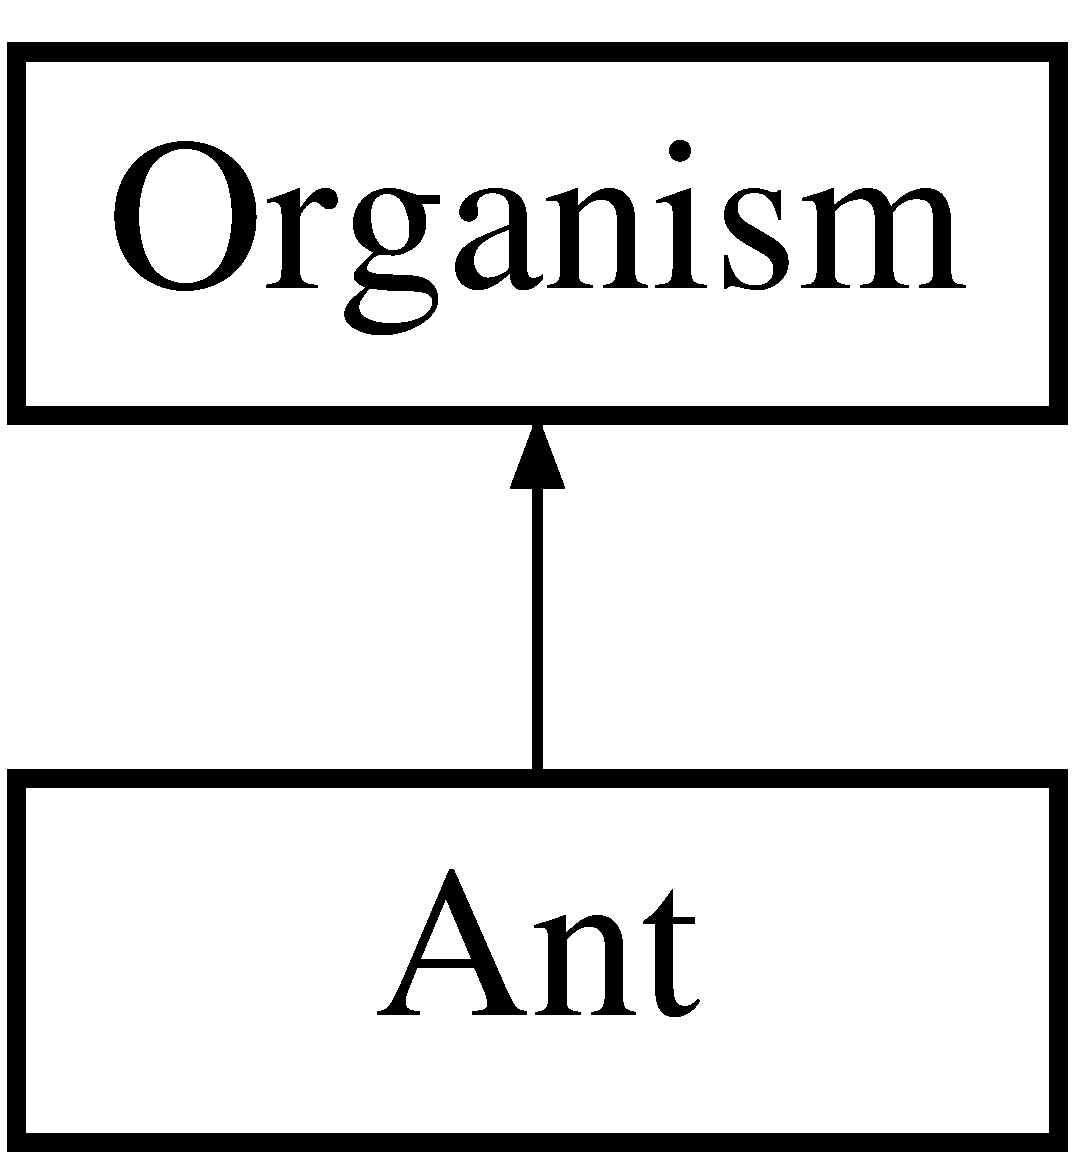
\includegraphics[height=2.000000cm]{classAnt}
\end{center}
\end{figure}
\subsection*{Public Member Functions}
\begin{DoxyCompactItemize}
\item 
\textbf{ Ant} (int r=0, int c=0)
\item 
bool \textbf{ move} (\textbf{ Cell} $\ast$new\+Cell)
\item 
bool \textbf{ breed} (\textbf{ Cell} $\ast$new\+Cell)
\item 
int \textbf{ get\+Row} ()
\item 
int \textbf{ get\+Col} ()
\item 
\textbf{ $\sim$\+Ant} ()
\end{DoxyCompactItemize}
\subsection*{Private Attributes}
\begin{DoxyCompactItemize}
\item 
int \textbf{ row} = 0
\item 
int \textbf{ col} = 0
\end{DoxyCompactItemize}
\subsection*{Additional Inherited Members}


\subsection{Detailed Description}
The \doxyref{Ant}{p.}{classAnt} class is a subclass of the \doxyref{Organism}{p.}{classOrganism} class, and is eligable to breed after it is alive for 3 timesteps, can be eaten by doodlebugs, and only moves into unoccupied cells. 

\subsection{Constructor \& Destructor Documentation}
\mbox{\label{classAnt_afcb9b285a5aa4b329e7eb5783970d85f}} 
\index{Ant@{Ant}!Ant@{Ant}}
\index{Ant@{Ant}!Ant@{Ant}}
\subsubsection{Ant()}
{\footnotesize\ttfamily Ant\+::\+Ant (\begin{DoxyParamCaption}\item[{int}]{r = {\ttfamily 0},  }\item[{int}]{c = {\ttfamily 0} }\end{DoxyParamCaption})}

Creates a new ant, which is also an organism 
\begin{DoxyParams}{Parameters}
{\em r} & the row this ant resides in \\
\hline
{\em c} & the column this ant resides in \\
\hline
\end{DoxyParams}


References col, row, and Organism\+::time\+Steps\+Survived.

\mbox{\label{classAnt_a33ca6bd592236726a18a2159908e4116}} 
\index{Ant@{Ant}!````~Ant@{$\sim$\+Ant}}
\index{````~Ant@{$\sim$\+Ant}!Ant@{Ant}}
\subsubsection{$\sim$\+Ant()}
{\footnotesize\ttfamily Ant\+::$\sim$\+Ant (\begin{DoxyParamCaption}{ }\end{DoxyParamCaption})}

Destroys the instance of the ant class 

Referenced by Tests2\+::test\+Ant\+Breed(), and Tests2\+::test\+Ant\+Move().



\subsection{Member Function Documentation}
\mbox{\label{classAnt_a083301b2522ea5fce044adcd8b442e14}} 
\index{Ant@{Ant}!breed@{breed}}
\index{breed@{breed}!Ant@{Ant}}
\subsubsection{breed()}
{\footnotesize\ttfamily bool Ant\+::breed (\begin{DoxyParamCaption}\item[{\textbf{ Cell} $\ast$}]{new\+Cell }\end{DoxyParamCaption})\hspace{0.3cm}{\ttfamily [virtual]}}

Breeds a new ant into the cell denoted by new\+Cell if the ant is eligable to breed. 
\begin{DoxyParams}{Parameters}
{\em new\+Cell} & the cell to breed into \\
\hline
\end{DoxyParams}
\begin{DoxyReturn}{Returns}
true if bred, false if it didn\textquotesingle{}t 
\end{DoxyReturn}


Implements \textbf{ Organism} \doxyref{}{p.}{classOrganism_a049af9fd24e663d524c21f0e6863e9a9}.



References ant, empty, Cell\+::get\+Cell\+Owner(), Cell\+::set\+Occupant(), Organism\+::set\+Step\+Ran(), and Organism\+::time\+Steps\+Survived.



Referenced by Tests2\+::test\+Ant\+Breed().

\mbox{\label{classAnt_a3c31dc577ebf913d246c16db3b1ed8e2}} 
\index{Ant@{Ant}!get\+Col@{get\+Col}}
\index{get\+Col@{get\+Col}!Ant@{Ant}}
\subsubsection{get\+Col()}
{\footnotesize\ttfamily int Ant\+::get\+Col (\begin{DoxyParamCaption}{ }\end{DoxyParamCaption})\hspace{0.3cm}{\ttfamily [virtual]}}

Gets the column that this ant resides in \begin{DoxyReturn}{Returns}
the column 
\end{DoxyReturn}


Implements \textbf{ Organism} \doxyref{}{p.}{classOrganism_ad61a864b21048f8304676a00d5c52800}.



References col.



Referenced by move(), and Tests2\+::test\+Ant\+Move().

\mbox{\label{classAnt_acef79a2f69e2493dc3067db4b41783a9}} 
\index{Ant@{Ant}!get\+Row@{get\+Row}}
\index{get\+Row@{get\+Row}!Ant@{Ant}}
\subsubsection{get\+Row()}
{\footnotesize\ttfamily int Ant\+::get\+Row (\begin{DoxyParamCaption}{ }\end{DoxyParamCaption})\hspace{0.3cm}{\ttfamily [virtual]}}

Gets the row that this ant resides in \begin{DoxyReturn}{Returns}
the row 
\end{DoxyReturn}


Implements \textbf{ Organism} \doxyref{}{p.}{classOrganism_a70700de2afe1358078cbc83581663096}.



References row.



Referenced by Tests2\+::test\+Ant\+Move().

\mbox{\label{classAnt_acf414aad7c33adf645f86d4a0a8523b4}} 
\index{Ant@{Ant}!move@{move}}
\index{move@{move}!Ant@{Ant}}
\subsubsection{move()}
{\footnotesize\ttfamily bool Ant\+::move (\begin{DoxyParamCaption}\item[{\textbf{ Cell} $\ast$}]{new\+Cell }\end{DoxyParamCaption})\hspace{0.3cm}{\ttfamily [virtual]}}

Moves the ant to the cell specified N\+O\+TE\+: The user must remove this ant from its current cell $\sim$before$\sim$ moving it to the new cell, as the ant itself does not keep track of what cell it is in, that is the grid\textquotesingle{}s job 
\begin{DoxyParams}{Parameters}
{\em new\+Cell} & the new cell to put the ant in \\
\hline
\end{DoxyParams}
\begin{DoxyReturn}{Returns}
true if move, false if fail 
\end{DoxyReturn}


Implements \textbf{ Organism} \doxyref{}{p.}{classOrganism_a79604b094754b64cea38a6eaf3ac36dc}.



References ant, col, empty, get\+Col(), Cell\+::get\+Occupant(), Cell\+::get\+Row(), row, Cell\+::set\+Occupant(), Cell\+::set\+Organism(), Organism\+::step\+Ran, and Organism\+::time\+Steps\+Survived.



Referenced by Tests2\+::test\+Ant\+Breed(), and Tests2\+::test\+Ant\+Move().



\subsection{Field Documentation}
\mbox{\label{classAnt_afe21bedec87ea26e3db74857960a78c6}} 
\index{Ant@{Ant}!col@{col}}
\index{col@{col}!Ant@{Ant}}
\subsubsection{col}
{\footnotesize\ttfamily int Ant\+::col = 0\hspace{0.3cm}{\ttfamily [private]}}



Referenced by Ant(), get\+Col(), and move().

\mbox{\label{classAnt_abf712c4a02e999938c7d79557a8fc24b}} 
\index{Ant@{Ant}!row@{row}}
\index{row@{row}!Ant@{Ant}}
\subsubsection{row}
{\footnotesize\ttfamily int Ant\+::row = 0\hspace{0.3cm}{\ttfamily [private]}}



Referenced by Ant(), get\+Row(), and move().



The documentation for this class was generated from the following files\+:\begin{DoxyCompactItemize}
\item 
\textbf{ Ant.\+h}\item 
\textbf{ Ant.\+cpp}\end{DoxyCompactItemize}

\section{Cell Class Reference}
\label{classCell}\index{Cell@{Cell}}


{\ttfamily \#include $<$Cell.\+h$>$}

\subsection*{Public Member Functions}
\begin{DoxyCompactItemize}
\item 
\textbf{ Cell} ()
\item 
void \textbf{ set\+Position} (int r, int c)
\item 
bool \textbf{ set\+Occupant} (\textbf{ occupation\+Status} g)
\item 
\textbf{ occupation\+Status} \textbf{ get\+Occupant} ()
\item 
\textbf{ Organism} $\ast$ \textbf{ get\+Cell\+Owner} ()
\item 
virtual \textbf{ $\sim$\+Cell} ()
\item 
void \textbf{ set\+Organism} (\textbf{ Organism} $\ast$set)
\item 
int \textbf{ get\+Row} ()
\item 
int \textbf{ get\+Col} ()
\end{DoxyCompactItemize}
\subsection*{Private Attributes}
\begin{DoxyCompactItemize}
\item 
\textbf{ occupation\+Status} \textbf{ guest}
\item 
\textbf{ Organism} $\ast$ \textbf{ guy}
\item 
int \textbf{ row}
\item 
int \textbf{ column}
\end{DoxyCompactItemize}


\subsection{Detailed Description}
The cell class contains the organism that is at the position in the grid, as well as the type of organism that is in it. 

\subsection{Constructor \& Destructor Documentation}
\mbox{\label{classCell_a394510643e8664cf12b5efaf5cb99f71}} 
\index{Cell@{Cell}!Cell@{Cell}}
\index{Cell@{Cell}!Cell@{Cell}}
\subsubsection{Cell()}
{\footnotesize\ttfamily Cell\+::\+Cell (\begin{DoxyParamCaption}{ }\end{DoxyParamCaption})}

Creates a new cell 

References column, empty, guest, guy, and row.

\mbox{\label{classCell_a9fa559f7a28e2b4336c6879ca09304d8}} 
\index{Cell@{Cell}!````~Cell@{$\sim$\+Cell}}
\index{````~Cell@{$\sim$\+Cell}!Cell@{Cell}}
\subsubsection{$\sim$\+Cell()}
{\footnotesize\ttfamily Cell\+::$\sim$\+Cell (\begin{DoxyParamCaption}{ }\end{DoxyParamCaption})\hspace{0.3cm}{\ttfamily [virtual]}}

Destroys the instance of this cell. 

Referenced by Tests2\+::test\+Ant\+Breed(), Tests2\+::test\+Ant\+Move(), Tests2\+::test\+Doodlebug\+Breed(), Tests2\+::test\+Doodlebug\+Move(), and Tests2\+::test\+Doodlebug\+Starve().



\subsection{Member Function Documentation}
\mbox{\label{classCell_a108ebd49b69b5cad9fcc27323d162058}} 
\index{Cell@{Cell}!get\+Cell\+Owner@{get\+Cell\+Owner}}
\index{get\+Cell\+Owner@{get\+Cell\+Owner}!Cell@{Cell}}
\subsubsection{get\+Cell\+Owner()}
{\footnotesize\ttfamily \textbf{ Organism} $\ast$ Cell\+::get\+Cell\+Owner (\begin{DoxyParamCaption}{ }\end{DoxyParamCaption})}

Returns a pointer to the organism that this cell represents. \begin{DoxyReturn}{Returns}
the organism that resides in this cell 
\end{DoxyReturn}


References guy.



Referenced by Doodlebug\+::breed(), Ant\+::breed(), and Grid\+::run().

\mbox{\label{classCell_ace419ef9ac6690bab2dd554d8b9f0d2f}} 
\index{Cell@{Cell}!get\+Col@{get\+Col}}
\index{get\+Col@{get\+Col}!Cell@{Cell}}
\subsubsection{get\+Col()}
{\footnotesize\ttfamily int Cell\+::get\+Col (\begin{DoxyParamCaption}{ }\end{DoxyParamCaption})}

Gets the column of this cell \begin{DoxyReturn}{Returns}
the column 
\end{DoxyReturn}


References column.



Referenced by Grid\+::run(), Tests2\+::test\+Ant\+Move(), Tests2\+::test\+Doodlebug\+Move(), and Grid\+::test\+Find\+Empty\+Cell().

\mbox{\label{classCell_a7dcb8bc75a2e2591b3fd52b5f7c28ab1}} 
\index{Cell@{Cell}!get\+Occupant@{get\+Occupant}}
\index{get\+Occupant@{get\+Occupant}!Cell@{Cell}}
\subsubsection{get\+Occupant()}
{\footnotesize\ttfamily \textbf{ occupation\+Status} Cell\+::get\+Occupant (\begin{DoxyParamCaption}{ }\end{DoxyParamCaption})}

Returns the occupation status of this cell \begin{DoxyReturn}{Returns}
empty, ant, or doodlebug 
\end{DoxyReturn}


References guest.



Referenced by Grid\+::get\+Cell\+Occupant(), Doodlebug\+::move(), Ant\+::move(), Grid\+::print\+Grid(), Grid\+::run(), Tests2\+::test\+Ant\+Breed(), Tests2\+::test\+Ant\+Move(), Tests2\+::test\+Doodlebug\+Breed(), and Tests2\+::test\+Doodlebug\+Move().

\mbox{\label{classCell_a6665d7f040a6a7b140e8d27c608a421e}} 
\index{Cell@{Cell}!get\+Row@{get\+Row}}
\index{get\+Row@{get\+Row}!Cell@{Cell}}
\subsubsection{get\+Row()}
{\footnotesize\ttfamily int Cell\+::get\+Row (\begin{DoxyParamCaption}{ }\end{DoxyParamCaption})}

Gets the row of this cell \begin{DoxyReturn}{Returns}
the row 
\end{DoxyReturn}


References row.



Referenced by Doodlebug\+::move(), Ant\+::move(), Grid\+::run(), Tests2\+::test\+Ant\+Move(), Tests2\+::test\+Doodlebug\+Move(), and Grid\+::test\+Find\+Empty\+Cell().

\mbox{\label{classCell_a2346933316b45d87264d50e563c2f895}} 
\index{Cell@{Cell}!set\+Occupant@{set\+Occupant}}
\index{set\+Occupant@{set\+Occupant}!Cell@{Cell}}
\subsubsection{set\+Occupant()}
{\footnotesize\ttfamily bool Cell\+::set\+Occupant (\begin{DoxyParamCaption}\item[{\textbf{ occupation\+Status}}]{g }\end{DoxyParamCaption})}

Sets the occupant type of this cell Setting it to ant will create a new ant in the organism space Setting it to doodlebug will create a new doodlebug in the organism space Setting it to empty will get rid of the entity in the organism space 
\begin{DoxyParams}{Parameters}
{\em g} & the occupation status that this cell will take on \\
\hline
\end{DoxyParams}
\begin{DoxyReturn}{Returns}
true 
\end{DoxyReturn}


References ant, column, doodlebug, empty, guest, guy, and row.



Referenced by Doodlebug\+::breed(), Ant\+::breed(), Doodlebug\+::move(), Ant\+::move(), Grid\+::run(), Grid\+::set\+Cell\+Occupant(), and Grid\+::set\+Up\+Grid().

\mbox{\label{classCell_afddad403027fbb6e2338776cf8e0be64}} 
\index{Cell@{Cell}!set\+Organism@{set\+Organism}}
\index{set\+Organism@{set\+Organism}!Cell@{Cell}}
\subsubsection{set\+Organism()}
{\footnotesize\ttfamily void Cell\+::set\+Organism (\begin{DoxyParamCaption}\item[{\textbf{ Organism} $\ast$}]{set }\end{DoxyParamCaption})}

Sets the organism of this cell to a certain organism 
\begin{DoxyParams}{Parameters}
{\em set} & the organism to let live in this cell \\
\hline
\end{DoxyParams}


References guy.



Referenced by Doodlebug\+::move(), and Ant\+::move().

\mbox{\label{classCell_adb03c2c5ee34982692b2375777a5d1cd}} 
\index{Cell@{Cell}!set\+Position@{set\+Position}}
\index{set\+Position@{set\+Position}!Cell@{Cell}}
\subsubsection{set\+Position()}
{\footnotesize\ttfamily void Cell\+::set\+Position (\begin{DoxyParamCaption}\item[{int}]{r,  }\item[{int}]{c }\end{DoxyParamCaption})}

Sets the position of this cell to a certain row and column 
\begin{DoxyParams}{Parameters}
{\em r} & the row of this cell \\
\hline
{\em c} & the column of this cell \\
\hline
\end{DoxyParams}


References column, and row.



Referenced by Grid\+::\+Grid(), Tests2\+::test\+Ant\+Breed(), Tests2\+::test\+Ant\+Move(), Tests2\+::test\+Doodlebug\+Breed(), Tests2\+::test\+Doodlebug\+Move(), and Tests2\+::test\+Doodlebug\+Starve().



\subsection{Field Documentation}
\mbox{\label{classCell_a6aae9428106f7cd7574660e3c2278ee0}} 
\index{Cell@{Cell}!column@{column}}
\index{column@{column}!Cell@{Cell}}
\subsubsection{column}
{\footnotesize\ttfamily int Cell\+::column\hspace{0.3cm}{\ttfamily [private]}}



Referenced by Cell(), get\+Col(), set\+Occupant(), and set\+Position().

\mbox{\label{classCell_aafc273a5125cf29742a8df6f5a5a881c}} 
\index{Cell@{Cell}!guest@{guest}}
\index{guest@{guest}!Cell@{Cell}}
\subsubsection{guest}
{\footnotesize\ttfamily \textbf{ occupation\+Status} Cell\+::guest\hspace{0.3cm}{\ttfamily [private]}}



Referenced by Cell(), get\+Occupant(), and set\+Occupant().

\mbox{\label{classCell_a3620f64df751ce23697f6cac13dfc151}} 
\index{Cell@{Cell}!guy@{guy}}
\index{guy@{guy}!Cell@{Cell}}
\subsubsection{guy}
{\footnotesize\ttfamily \textbf{ Organism}$\ast$ Cell\+::guy\hspace{0.3cm}{\ttfamily [private]}}



Referenced by Cell(), get\+Cell\+Owner(), set\+Occupant(), and set\+Organism().

\mbox{\label{classCell_a85d2a7af6195f5196574790fbc1becfd}} 
\index{Cell@{Cell}!row@{row}}
\index{row@{row}!Cell@{Cell}}
\subsubsection{row}
{\footnotesize\ttfamily int Cell\+::row\hspace{0.3cm}{\ttfamily [private]}}



Referenced by Cell(), get\+Row(), set\+Occupant(), and set\+Position().



The documentation for this class was generated from the following files\+:\begin{DoxyCompactItemize}
\item 
\textbf{ Cell.\+h}\item 
\textbf{ Cell.\+cpp}\end{DoxyCompactItemize}

\section{Doodlebug Class Reference}
\label{classDoodlebug}\index{Doodlebug@{Doodlebug}}


{\ttfamily \#include $<$Doodlebug.\+h$>$}

Inheritance diagram for Doodlebug\+:\begin{figure}[H]
\begin{center}
\leavevmode
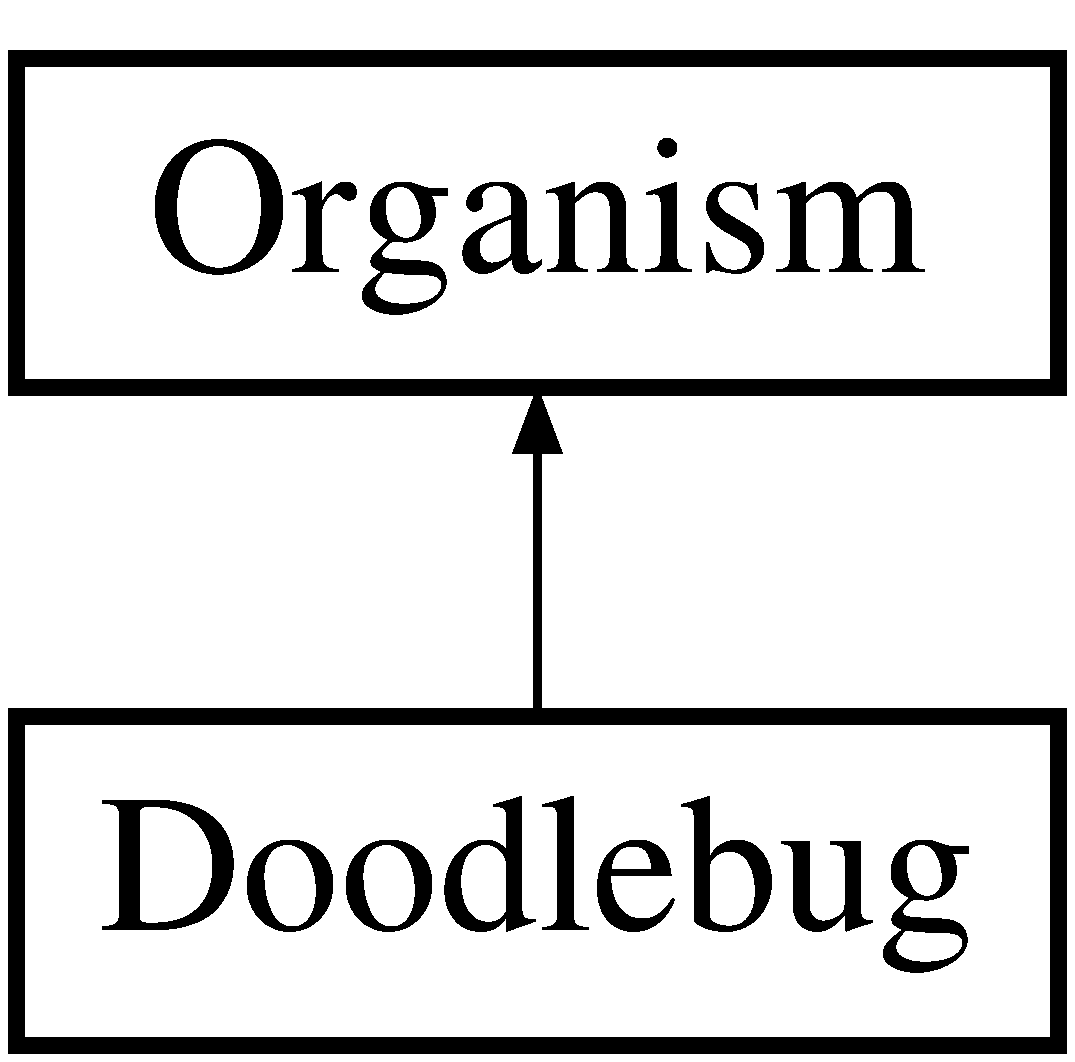
\includegraphics[height=2.000000cm]{classDoodlebug}
\end{center}
\end{figure}
\subsection*{Public Member Functions}
\begin{DoxyCompactItemize}
\item 
\textbf{ Doodlebug} (int r, int c)
\item 
bool \textbf{ move} (\textbf{ Cell} $\ast$new\+Cell)
\item 
bool \textbf{ breed} (\textbf{ Cell} $\ast$new\+Cell)
\item 
bool \textbf{ starve} ()
\item 
int \textbf{ get\+Row} ()
\item 
int \textbf{ get\+Col} ()
\item 
\textbf{ $\sim$\+Doodlebug} ()
\end{DoxyCompactItemize}
\subsection*{Private Attributes}
\begin{DoxyCompactItemize}
\item 
int \textbf{ row}
\item 
int \textbf{ column}
\item 
int \textbf{ steps\+Without\+Eating} = 0
\end{DoxyCompactItemize}
\subsection*{Additional Inherited Members}


\subsection{Detailed Description}
The doodlebug class is a subclass of the \doxyref{Organism}{p.}{classOrganism} class, is eligable to breed after surviving 8 turns, can starve after not eating for 3 turns, can eat ants by moving into the cell that they are in, and will always move before the ants. 

\subsection{Constructor \& Destructor Documentation}
\mbox{\label{classDoodlebug_a0009927ec98eb6203900af3637fb3e3a}} 
\index{Doodlebug@{Doodlebug}!Doodlebug@{Doodlebug}}
\index{Doodlebug@{Doodlebug}!Doodlebug@{Doodlebug}}
\subsubsection{Doodlebug()}
{\footnotesize\ttfamily Doodlebug\+::\+Doodlebug (\begin{DoxyParamCaption}\item[{int}]{r,  }\item[{int}]{c }\end{DoxyParamCaption})}

Creates a new \doxyref{Doodlebug}{p.}{classDoodlebug}, which is also an \doxyref{Organism}{p.}{classOrganism} 
\begin{DoxyParams}{Parameters}
{\em r} & the row that this doodlebug resides in \\
\hline
{\em c} & the column that this doodlebug resides in \\
\hline
\end{DoxyParams}


References column, row, and Organism\+::time\+Steps\+Survived.

\mbox{\label{classDoodlebug_ac318cc9acbd9a3af52348a236070d891}} 
\index{Doodlebug@{Doodlebug}!````~Doodlebug@{$\sim$\+Doodlebug}}
\index{````~Doodlebug@{$\sim$\+Doodlebug}!Doodlebug@{Doodlebug}}
\subsubsection{$\sim$\+Doodlebug()}
{\footnotesize\ttfamily Doodlebug\+::$\sim$\+Doodlebug (\begin{DoxyParamCaption}{ }\end{DoxyParamCaption})}

Destroys the doodlebug instance. 

Referenced by Tests2\+::test\+Doodlebug\+Breed(), Tests2\+::test\+Doodlebug\+Move(), and Tests2\+::test\+Doodlebug\+Starve().



\subsection{Member Function Documentation}
\mbox{\label{classDoodlebug_a619223ecb7063d9bbd88c53105dfab64}} 
\index{Doodlebug@{Doodlebug}!breed@{breed}}
\index{breed@{breed}!Doodlebug@{Doodlebug}}
\subsubsection{breed()}
{\footnotesize\ttfamily bool Doodlebug\+::breed (\begin{DoxyParamCaption}\item[{\textbf{ Cell} $\ast$}]{new\+Cell }\end{DoxyParamCaption})\hspace{0.3cm}{\ttfamily [virtual]}}

Breeds a new doodlebug into the cell denoted by new\+Cell if the doodlebug is eligable to breed. 
\begin{DoxyParams}{Parameters}
{\em new\+Cell} & the cell to breed into \\
\hline
\end{DoxyParams}
\begin{DoxyReturn}{Returns}
true if bred, false if it didn\textquotesingle{}t 
\end{DoxyReturn}


Implements \textbf{ Organism} \doxyref{}{p.}{classOrganism_a049af9fd24e663d524c21f0e6863e9a9}.



References doodlebug, empty, Cell\+::get\+Cell\+Owner(), Cell\+::set\+Occupant(), Organism\+::set\+Step\+Ran(), and Organism\+::time\+Steps\+Survived.



Referenced by Tests2\+::test\+Doodlebug\+Breed().

\mbox{\label{classDoodlebug_aa311d47bffaf0e68785b8a1472537807}} 
\index{Doodlebug@{Doodlebug}!get\+Col@{get\+Col}}
\index{get\+Col@{get\+Col}!Doodlebug@{Doodlebug}}
\subsubsection{get\+Col()}
{\footnotesize\ttfamily int Doodlebug\+::get\+Col (\begin{DoxyParamCaption}{ }\end{DoxyParamCaption})\hspace{0.3cm}{\ttfamily [virtual]}}

Gets the column of the cell that this doodlebug resides in \begin{DoxyReturn}{Returns}
the column 
\end{DoxyReturn}


Implements \textbf{ Organism} \doxyref{}{p.}{classOrganism_ad61a864b21048f8304676a00d5c52800}.



References column.



Referenced by move(), and Tests2\+::test\+Doodlebug\+Move().

\mbox{\label{classDoodlebug_afb3ba6dc552b2c83caf316405db616ec}} 
\index{Doodlebug@{Doodlebug}!get\+Row@{get\+Row}}
\index{get\+Row@{get\+Row}!Doodlebug@{Doodlebug}}
\subsubsection{get\+Row()}
{\footnotesize\ttfamily int Doodlebug\+::get\+Row (\begin{DoxyParamCaption}{ }\end{DoxyParamCaption})\hspace{0.3cm}{\ttfamily [virtual]}}

Gets the row of the cell that this doodlebug resides in \begin{DoxyReturn}{Returns}
the row 
\end{DoxyReturn}


Implements \textbf{ Organism} \doxyref{}{p.}{classOrganism_a70700de2afe1358078cbc83581663096}.



References row.



Referenced by Tests2\+::test\+Doodlebug\+Move().

\mbox{\label{classDoodlebug_a779e9b9fb85a8ef9814ae0d1e800d971}} 
\index{Doodlebug@{Doodlebug}!move@{move}}
\index{move@{move}!Doodlebug@{Doodlebug}}
\subsubsection{move()}
{\footnotesize\ttfamily bool Doodlebug\+::move (\begin{DoxyParamCaption}\item[{\textbf{ Cell} $\ast$}]{new\+Cell }\end{DoxyParamCaption})\hspace{0.3cm}{\ttfamily [virtual]}}

Moves the doodlebug to the cell specified N\+O\+TE\+: The user must remove this doodlebug from its current cell $\sim$before$\sim$ moving it to the new cell, as the doodlebug itself does not keep track of what cell it is in, that is the grid\textquotesingle{}s job 
\begin{DoxyParams}{Parameters}
{\em new\+Cell} & the new cell to put the doodlebug in \\
\hline
\end{DoxyParams}
\begin{DoxyReturn}{Returns}
true, it will not fail to move. 
\end{DoxyReturn}


Implements \textbf{ Organism} \doxyref{}{p.}{classOrganism_a79604b094754b64cea38a6eaf3ac36dc}.



References ant, column, doodlebug, get\+Col(), Cell\+::get\+Occupant(), Cell\+::get\+Row(), row, Cell\+::set\+Occupant(), Cell\+::set\+Organism(), Organism\+::step\+Ran, steps\+Without\+Eating, and Organism\+::time\+Steps\+Survived.



Referenced by Tests2\+::test\+Doodlebug\+Breed(), Tests2\+::test\+Doodlebug\+Move(), and Tests2\+::test\+Doodlebug\+Starve().

\mbox{\label{classDoodlebug_a7f1c26c8458f3811680c778362c0e374}} 
\index{Doodlebug@{Doodlebug}!starve@{starve}}
\index{starve@{starve}!Doodlebug@{Doodlebug}}
\subsubsection{starve()}
{\footnotesize\ttfamily bool Doodlebug\+::starve (\begin{DoxyParamCaption}{ }\end{DoxyParamCaption})}

Checks to see if the doodlebug starves N\+O\+TE\+: The user must deal with actually killing off the doodlebug, as this only checks to see if the doodlebug is eligable to starve. \begin{DoxyReturn}{Returns}
true if the doodlebug will starve, false if it is fine 
\end{DoxyReturn}


References steps\+Without\+Eating.



Referenced by Grid\+::run(), and Tests2\+::test\+Doodlebug\+Starve().



\subsection{Field Documentation}
\mbox{\label{classDoodlebug_ac3a53739f9b05a793724a78c2bd29e69}} 
\index{Doodlebug@{Doodlebug}!column@{column}}
\index{column@{column}!Doodlebug@{Doodlebug}}
\subsubsection{column}
{\footnotesize\ttfamily int Doodlebug\+::column\hspace{0.3cm}{\ttfamily [private]}}



Referenced by Doodlebug(), get\+Col(), and move().

\mbox{\label{classDoodlebug_a4ab3657542999f3f83988ff1e113d477}} 
\index{Doodlebug@{Doodlebug}!row@{row}}
\index{row@{row}!Doodlebug@{Doodlebug}}
\subsubsection{row}
{\footnotesize\ttfamily int Doodlebug\+::row\hspace{0.3cm}{\ttfamily [private]}}



Referenced by Doodlebug(), get\+Row(), move(), and Grid\+::set\+Up\+Grid().

\mbox{\label{classDoodlebug_a440e97dfc162db5fab4d632aab30f266}} 
\index{Doodlebug@{Doodlebug}!steps\+Without\+Eating@{steps\+Without\+Eating}}
\index{steps\+Without\+Eating@{steps\+Without\+Eating}!Doodlebug@{Doodlebug}}
\subsubsection{steps\+Without\+Eating}
{\footnotesize\ttfamily int Doodlebug\+::steps\+Without\+Eating = 0\hspace{0.3cm}{\ttfamily [private]}}



Referenced by move(), and starve().



The documentation for this class was generated from the following files\+:\begin{DoxyCompactItemize}
\item 
\textbf{ Doodlebug.\+h}\item 
\textbf{ Doodlebug.\+cpp}\end{DoxyCompactItemize}

\section{Grid Class Reference}
\label{classGrid}\index{Grid@{Grid}}


{\ttfamily \#include $<$Grid.\+h$>$}

\subsection*{Public Member Functions}
\begin{DoxyCompactItemize}
\item 
\textbf{ Grid} (int n\+Squares\+On\+A\+Side=20, int doodlebugs=5, int ants=100, int g=1000, int seed=1, int \textbf{ pause}=0)
\item 
virtual \textbf{ $\sim$\+Grid} ()
\item 
int \textbf{ run} ()
\item 
int \textbf{ get\+Ant\+Count} ()
\item 
int \textbf{ get\+Doodle\+Count} ()
\item 
void \textbf{ print\+Grid} ()
\end{DoxyCompactItemize}
\subsection*{Static Public Member Functions}
\begin{DoxyCompactItemize}
\item 
static bool \textbf{ test\+Find\+Empty\+Cell} ()
\item 
static bool \textbf{ test\+Valid\+Location} ()
\item 
static bool \textbf{ test\+Get\+Set\+Occupant} ()
\end{DoxyCompactItemize}
\subsection*{Private Member Functions}
\begin{DoxyCompactItemize}
\item 
void \textbf{ set\+Up\+Grid} (int number, \textbf{ occupation\+Status} to\+Set\+Up)
\item 
\textbf{ Cell} $\ast$ \textbf{ find\+Open\+Cell} (int r, int c, \textbf{ occupation\+Status} to\+Look\+For)
\item 
bool \textbf{ is\+Valid\+Location} (int r, int c)
\item 
bool \textbf{ set\+Cell\+Occupant} (int r, int c, \textbf{ occupation\+Status} g)
\item 
\textbf{ occupation\+Status} \textbf{ get\+Cell\+Occupant} (int r, int c)
\end{DoxyCompactItemize}
\subsection*{Private Attributes}
\begin{DoxyCompactItemize}
\item 
int \textbf{ size\+Of\+Grid}
\item 
int \textbf{ gens}
\item 
int \textbf{ doodle\+Left}
\item 
int \textbf{ ants\+Left}
\item 
bool \textbf{ pause}
\item 
\textbf{ Cell} $\ast$$\ast$ \textbf{ my\+Grid\+Cells\+\_\+ptr\+\_\+array} = nullptr
\end{DoxyCompactItemize}


\subsection{Detailed Description}
The grid class contains the grid for the simulation, and handles running all of the calculations for the simulation as well. 

\subsection{Constructor \& Destructor Documentation}
\mbox{\label{classGrid_a9fba66bc1c663e166ee5ddbe8cc99648}} 
\index{Grid@{Grid}!Grid@{Grid}}
\index{Grid@{Grid}!Grid@{Grid}}
\subsubsection{Grid()}
{\footnotesize\ttfamily Grid\+::\+Grid (\begin{DoxyParamCaption}\item[{int}]{n\+Squares\+On\+A\+Side = {\ttfamily 20},  }\item[{int}]{doodlebugs = {\ttfamily 5},  }\item[{int}]{ants = {\ttfamily 100},  }\item[{int}]{g = {\ttfamily 1000},  }\item[{int}]{seed = {\ttfamily 1},  }\item[{int}]{stop = {\ttfamily 0} }\end{DoxyParamCaption})}

Constructs a new grid 
\begin{DoxyParams}{Parameters}
{\em n\+Squares\+On\+A\+Side} & the diameter of the board, default is 20 \\
\hline
{\em doodlebugs} & the number of doodlebugs on the board, default is 5 \\
\hline
{\em ants} & the number of ants on the board, default is 100 \\
\hline
{\em g} & the number of generations to run, default is 1000 \\
\hline
{\em seed} & the seed to use when randomly generating the board, default is 1 \\
\hline
{\em stop} & if nonzero, then the program waits for user input before running another generation. default is 0. \\
\hline
\end{DoxyParams}


References ant, ants\+Left, doodlebug, doodle\+Left, gens, my\+Grid\+Cells\+\_\+ptr\+\_\+array, pause, Cell\+::set\+Position(), set\+Up\+Grid(), and size\+Of\+Grid.



Referenced by test\+Find\+Empty\+Cell(), test\+Get\+Set\+Occupant(), and test\+Valid\+Location().

\mbox{\label{classGrid_a3661d0a7f998caaaf8627d7a67072116}} 
\index{Grid@{Grid}!````~Grid@{$\sim$\+Grid}}
\index{````~Grid@{$\sim$\+Grid}!Grid@{Grid}}
\subsubsection{$\sim$\+Grid()}
{\footnotesize\ttfamily Grid\+::$\sim$\+Grid (\begin{DoxyParamCaption}{ }\end{DoxyParamCaption})\hspace{0.3cm}{\ttfamily [virtual]}}

Destroys this object. 

Referenced by Production\+::run\+Production(), Tests2\+::test\+Counting(), test\+Find\+Empty\+Cell(), test\+Get\+Set\+Occupant(), and test\+Valid\+Location().



\subsection{Member Function Documentation}
\mbox{\label{classGrid_a096354cc6efe278e84e1f83f58065f80}} 
\index{Grid@{Grid}!find\+Open\+Cell@{find\+Open\+Cell}}
\index{find\+Open\+Cell@{find\+Open\+Cell}!Grid@{Grid}}
\subsubsection{find\+Open\+Cell()}
{\footnotesize\ttfamily \textbf{ Cell} $\ast$ Grid\+::find\+Open\+Cell (\begin{DoxyParamCaption}\item[{int}]{r,  }\item[{int}]{c,  }\item[{\textbf{ occupation\+Status}}]{to\+Look\+For }\end{DoxyParamCaption})\hspace{0.3cm}{\ttfamily [private]}}

Finds a cell either below, above, to the right, or to the left of the cell denoted by r,c. It is looking for the type of cell denoted by the occupation status. 
\begin{DoxyParams}{Parameters}
{\em r} & the row of the cell to look around \\
\hline
{\em c} & the column of the cell to look around \\
\hline
{\em to\+Look\+For} & the type of cell we are looking for, either an empty one, ant one, or a doodlebug one \\
\hline
\end{DoxyParams}
\begin{DoxyReturn}{Returns}
a pointer to the cell that the function deems is an \char`\"{}open\char`\"{} cell based on the occupation\+Status. If the function does not find a cell, it will return a nullptr. 
\end{DoxyReturn}


References get\+Cell\+Occupant(), is\+Valid\+Location(), and my\+Grid\+Cells\+\_\+ptr\+\_\+array.



Referenced by run(), and test\+Find\+Empty\+Cell().

\mbox{\label{classGrid_ac4420d02072ef7d7298d85bf7d1b59f5}} 
\index{Grid@{Grid}!get\+Ant\+Count@{get\+Ant\+Count}}
\index{get\+Ant\+Count@{get\+Ant\+Count}!Grid@{Grid}}
\subsubsection{get\+Ant\+Count()}
{\footnotesize\ttfamily int Grid\+::get\+Ant\+Count (\begin{DoxyParamCaption}{ }\end{DoxyParamCaption})}

Gets the current number of ants on the board \begin{DoxyReturn}{Returns}
the amount of ants on the board 
\end{DoxyReturn}


References ants\+Left.



Referenced by Production\+::run\+Production(), and Tests2\+::test\+Counting().

\mbox{\label{classGrid_ae9f685fddd449805e372d59cfa6c42d6}} 
\index{Grid@{Grid}!get\+Cell\+Occupant@{get\+Cell\+Occupant}}
\index{get\+Cell\+Occupant@{get\+Cell\+Occupant}!Grid@{Grid}}
\subsubsection{get\+Cell\+Occupant()}
{\footnotesize\ttfamily \textbf{ occupation\+Status} Grid\+::get\+Cell\+Occupant (\begin{DoxyParamCaption}\item[{int}]{r,  }\item[{int}]{c }\end{DoxyParamCaption})\hspace{0.3cm}{\ttfamily [private]}}

Returns the cell occupant at the cell denoted by r,c 
\begin{DoxyParams}{Parameters}
{\em r} & the row of the cell \\
\hline
{\em c} & the column of the cell \\
\hline
\end{DoxyParams}
\begin{DoxyReturn}{Returns}
the occupation\+Status of that cell (either empty, ant, or doodlebug) 
\end{DoxyReturn}


References Cell\+::get\+Occupant(), and my\+Grid\+Cells\+\_\+ptr\+\_\+array.



Referenced by find\+Open\+Cell(), and test\+Get\+Set\+Occupant().

\mbox{\label{classGrid_a388390334f29ee7ba070eb59ca5d9608}} 
\index{Grid@{Grid}!get\+Doodle\+Count@{get\+Doodle\+Count}}
\index{get\+Doodle\+Count@{get\+Doodle\+Count}!Grid@{Grid}}
\subsubsection{get\+Doodle\+Count()}
{\footnotesize\ttfamily int Grid\+::get\+Doodle\+Count (\begin{DoxyParamCaption}{ }\end{DoxyParamCaption})}

Gets the current number of doodlebugs on the board \begin{DoxyReturn}{Returns}
the amount of doodlebugs on the board 
\end{DoxyReturn}


References doodle\+Left.



Referenced by Production\+::run\+Production(), and Tests2\+::test\+Counting().

\mbox{\label{classGrid_afd0c162988f2395c9a9555955e33b946}} 
\index{Grid@{Grid}!is\+Valid\+Location@{is\+Valid\+Location}}
\index{is\+Valid\+Location@{is\+Valid\+Location}!Grid@{Grid}}
\subsubsection{is\+Valid\+Location()}
{\footnotesize\ttfamily bool Grid\+::is\+Valid\+Location (\begin{DoxyParamCaption}\item[{int}]{r,  }\item[{int}]{c }\end{DoxyParamCaption})\hspace{0.3cm}{\ttfamily [private]}}

Checks to see if the row and column are valid locations on this grid 
\begin{DoxyParams}{Parameters}
{\em r} & the row to check \\
\hline
{\em c} & the column to check \\
\hline
\end{DoxyParams}
\begin{DoxyReturn}{Returns}
true if it is a valid point (0 $<$= r,c $<$ size\+Of\+Grid), false if not 
\end{DoxyReturn}


References size\+Of\+Grid.



Referenced by find\+Open\+Cell(), set\+Up\+Grid(), and test\+Valid\+Location().

\mbox{\label{classGrid_a04601ea9795a6928190e64fa89f10499}} 
\index{Grid@{Grid}!print\+Grid@{print\+Grid}}
\index{print\+Grid@{print\+Grid}!Grid@{Grid}}
\subsubsection{print\+Grid()}
{\footnotesize\ttfamily void Grid\+::print\+Grid (\begin{DoxyParamCaption}{ }\end{DoxyParamCaption})}

Prints the current state of the grid, with doodlebugs denoted as \char`\"{}x\char`\"{} and ants denoted as \char`\"{}o\char`\"{} 

References ant, doodlebug, Cell\+::get\+Occupant(), my\+Grid\+Cells\+\_\+ptr\+\_\+array, and size\+Of\+Grid.



Referenced by run(), Production\+::run\+Production(), Tests2\+::test\+Counting(), test\+Find\+Empty\+Cell(), and test\+Get\+Set\+Occupant().

\mbox{\label{classGrid_a00d51479ec5c4af0261a0dd3fb7a1000}} 
\index{Grid@{Grid}!run@{run}}
\index{run@{run}!Grid@{Grid}}
\subsubsection{run()}
{\footnotesize\ttfamily int Grid\+::run (\begin{DoxyParamCaption}{ }\end{DoxyParamCaption})}

Runs the grid for however many generations specified or until an end condition is met. \begin{DoxyReturn}{Returns}
the number of generations ran 
\end{DoxyReturn}


References ant, ants\+Left, Organism\+::breed(), doodlebug, doodle\+Left, empty, find\+Open\+Cell(), gens, Cell\+::get\+Cell\+Owner(), Cell\+::get\+Col(), Cell\+::get\+Occupant(), Cell\+::get\+Row(), Organism\+::get\+Step\+Ran(), Organism\+::move(), my\+Grid\+Cells\+\_\+ptr\+\_\+array, pause, print\+Grid(), Cell\+::set\+Occupant(), Organism\+::set\+Step\+Ran(), size\+Of\+Grid, Doodlebug\+::starve(), and Organism\+::$\sim$\+Organism().



Referenced by Production\+::run\+Production().

\mbox{\label{classGrid_ae74bcb1a42d969ece65fc00842715a8a}} 
\index{Grid@{Grid}!set\+Cell\+Occupant@{set\+Cell\+Occupant}}
\index{set\+Cell\+Occupant@{set\+Cell\+Occupant}!Grid@{Grid}}
\subsubsection{set\+Cell\+Occupant()}
{\footnotesize\ttfamily bool Grid\+::set\+Cell\+Occupant (\begin{DoxyParamCaption}\item[{int}]{r,  }\item[{int}]{c,  }\item[{\textbf{ occupation\+Status}}]{g }\end{DoxyParamCaption})\hspace{0.3cm}{\ttfamily [private]}}

Sets the occupant of the cell at r,c to be either an ant, doodlebug, or empty 
\begin{DoxyParams}{Parameters}
{\em r} & the row in the cell array \\
\hline
{\em c} & the column in the cell array \\
\hline
{\em g} & the status to set that cell to \\
\hline
\end{DoxyParams}
\begin{DoxyReturn}{Returns}
true if occupant set, false if fail 
\end{DoxyReturn}


References my\+Grid\+Cells\+\_\+ptr\+\_\+array, and Cell\+::set\+Occupant().



Referenced by test\+Find\+Empty\+Cell(), and test\+Get\+Set\+Occupant().

\mbox{\label{classGrid_afd6a52f97e4cde08d1c502fb7f6286b4}} 
\index{Grid@{Grid}!set\+Up\+Grid@{set\+Up\+Grid}}
\index{set\+Up\+Grid@{set\+Up\+Grid}!Grid@{Grid}}
\subsubsection{set\+Up\+Grid()}
{\footnotesize\ttfamily void Grid\+::set\+Up\+Grid (\begin{DoxyParamCaption}\item[{int}]{number,  }\item[{\textbf{ occupation\+Status}}]{to\+Set\+Up }\end{DoxyParamCaption})\hspace{0.3cm}{\ttfamily [private]}}

Sets up the grid with an amount of a certain occupation\+Status in random locations. 
\begin{DoxyParams}{Parameters}
{\em number} & the amount of entities to put on the grid \\
\hline
{\em to\+Set\+Up} & the kind of entity to put on the grid (ant or doodlebug?) \\
\hline
\end{DoxyParams}


References empty, is\+Valid\+Location(), my\+Grid\+Cells\+\_\+ptr\+\_\+array, Doodlebug\+::row, Cell\+::set\+Occupant(), and size\+Of\+Grid.



Referenced by Grid().

\mbox{\label{classGrid_a47784ddea186ff3349034695267edf4d}} 
\index{Grid@{Grid}!test\+Find\+Empty\+Cell@{test\+Find\+Empty\+Cell}}
\index{test\+Find\+Empty\+Cell@{test\+Find\+Empty\+Cell}!Grid@{Grid}}
\subsubsection{test\+Find\+Empty\+Cell()}
{\footnotesize\ttfamily static bool Grid\+::test\+Find\+Empty\+Cell (\begin{DoxyParamCaption}{ }\end{DoxyParamCaption})\hspace{0.3cm}{\ttfamily [inline]}, {\ttfamily [static]}}

Function to test whether find\+Empty\+Cell works \begin{DoxyReturn}{Returns}
true if find\+Empty\+Cell works, false if failed 
\end{DoxyReturn}


References ant, empty, find\+Open\+Cell(), Cell\+::get\+Col(), Cell\+::get\+Row(), Grid(), print\+Grid(), set\+Cell\+Occupant(), and $\sim$\+Grid().



Referenced by Tests2\+::do\+Tests().

\mbox{\label{classGrid_a48beaabc983c91a8acaff2d27b0c6623}} 
\index{Grid@{Grid}!test\+Get\+Set\+Occupant@{test\+Get\+Set\+Occupant}}
\index{test\+Get\+Set\+Occupant@{test\+Get\+Set\+Occupant}!Grid@{Grid}}
\subsubsection{test\+Get\+Set\+Occupant()}
{\footnotesize\ttfamily static bool Grid\+::test\+Get\+Set\+Occupant (\begin{DoxyParamCaption}{ }\end{DoxyParamCaption})\hspace{0.3cm}{\ttfamily [inline]}, {\ttfamily [static]}}

Tests to make sure that get\+Occupant and set\+Occupant in \doxyref{Grid}{p.}{classGrid} both work \begin{DoxyReturn}{Returns}
true if pass, false if fail 
\end{DoxyReturn}


References ant, doodlebug, empty, get\+Cell\+Occupant(), Grid(), print\+Grid(), set\+Cell\+Occupant(), and $\sim$\+Grid().



Referenced by Tests2\+::do\+Tests().

\mbox{\label{classGrid_afbeeff7ec70a7805220e703914255850}} 
\index{Grid@{Grid}!test\+Valid\+Location@{test\+Valid\+Location}}
\index{test\+Valid\+Location@{test\+Valid\+Location}!Grid@{Grid}}
\subsubsection{test\+Valid\+Location()}
{\footnotesize\ttfamily static bool Grid\+::test\+Valid\+Location (\begin{DoxyParamCaption}{ }\end{DoxyParamCaption})\hspace{0.3cm}{\ttfamily [inline]}, {\ttfamily [static]}}

Function to test whether is\+Valid\+Location works \begin{DoxyReturn}{Returns}
true if works, false if fail 
\end{DoxyReturn}


References Grid(), is\+Valid\+Location(), and $\sim$\+Grid().



Referenced by Tests2\+::do\+Tests().



\subsection{Field Documentation}
\mbox{\label{classGrid_a8a3929f044f6b68c9313fbd071ed3ab5}} 
\index{Grid@{Grid}!ants\+Left@{ants\+Left}}
\index{ants\+Left@{ants\+Left}!Grid@{Grid}}
\subsubsection{ants\+Left}
{\footnotesize\ttfamily int Grid\+::ants\+Left\hspace{0.3cm}{\ttfamily [private]}}



Referenced by get\+Ant\+Count(), Grid(), and run().

\mbox{\label{classGrid_add3c642b9a8924523b0ae1981f9ae4ad}} 
\index{Grid@{Grid}!doodle\+Left@{doodle\+Left}}
\index{doodle\+Left@{doodle\+Left}!Grid@{Grid}}
\subsubsection{doodle\+Left}
{\footnotesize\ttfamily int Grid\+::doodle\+Left\hspace{0.3cm}{\ttfamily [private]}}



Referenced by get\+Doodle\+Count(), Grid(), and run().

\mbox{\label{classGrid_a75d4728cd69d066c6c62ad7b67ff7cec}} 
\index{Grid@{Grid}!gens@{gens}}
\index{gens@{gens}!Grid@{Grid}}
\subsubsection{gens}
{\footnotesize\ttfamily int Grid\+::gens\hspace{0.3cm}{\ttfamily [private]}}



Referenced by Grid(), and run().

\mbox{\label{classGrid_a7b9fe8942b4ac7767c08bedfd66428ee}} 
\index{Grid@{Grid}!my\+Grid\+Cells\+\_\+ptr\+\_\+array@{my\+Grid\+Cells\+\_\+ptr\+\_\+array}}
\index{my\+Grid\+Cells\+\_\+ptr\+\_\+array@{my\+Grid\+Cells\+\_\+ptr\+\_\+array}!Grid@{Grid}}
\subsubsection{my\+Grid\+Cells\+\_\+ptr\+\_\+array}
{\footnotesize\ttfamily \textbf{ Cell}$\ast$$\ast$ Grid\+::my\+Grid\+Cells\+\_\+ptr\+\_\+array = nullptr\hspace{0.3cm}{\ttfamily [private]}}



Referenced by find\+Open\+Cell(), get\+Cell\+Occupant(), Grid(), print\+Grid(), run(), set\+Cell\+Occupant(), and set\+Up\+Grid().

\mbox{\label{classGrid_ad811dffc8e8ba3e58991f5f57b82e81a}} 
\index{Grid@{Grid}!pause@{pause}}
\index{pause@{pause}!Grid@{Grid}}
\subsubsection{pause}
{\footnotesize\ttfamily bool Grid\+::pause\hspace{0.3cm}{\ttfamily [private]}}



Referenced by Grid(), and run().

\mbox{\label{classGrid_aaa6ce6b1a451db2f752b360491a0fed9}} 
\index{Grid@{Grid}!size\+Of\+Grid@{size\+Of\+Grid}}
\index{size\+Of\+Grid@{size\+Of\+Grid}!Grid@{Grid}}
\subsubsection{size\+Of\+Grid}
{\footnotesize\ttfamily int Grid\+::size\+Of\+Grid\hspace{0.3cm}{\ttfamily [private]}}



Referenced by Grid(), is\+Valid\+Location(), print\+Grid(), run(), and set\+Up\+Grid().



The documentation for this class was generated from the following files\+:\begin{DoxyCompactItemize}
\item 
\textbf{ Grid.\+h}\item 
\textbf{ Grid.\+cpp}\end{DoxyCompactItemize}

\section{Organism Class Reference}
\label{classOrganism}\index{Organism@{Organism}}


{\ttfamily \#include $<$Organism.\+h$>$}

Inheritance diagram for Organism\+:\begin{figure}[H]
\begin{center}
\leavevmode
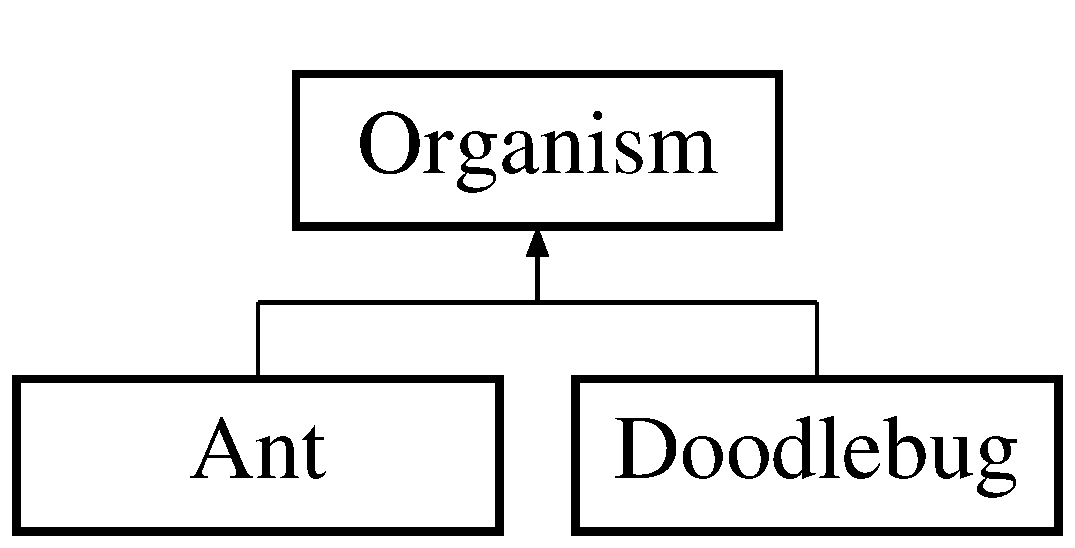
\includegraphics[height=2.000000cm]{classOrganism}
\end{center}
\end{figure}
\subsection*{Public Member Functions}
\begin{DoxyCompactItemize}
\item 
\textbf{ Organism} ()
\item 
virtual bool \textbf{ move} (\textbf{ Cell} $\ast$new\+Cell)=0
\item 
virtual bool \textbf{ breed} (\textbf{ Cell} $\ast$new\+Cell)=0
\item 
virtual int \textbf{ get\+Row} ()=0
\item 
virtual int \textbf{ get\+Col} ()=0
\item 
virtual \textbf{ $\sim$\+Organism} ()
\item 
void \textbf{ set\+Step\+Ran} (bool b)
\item 
bool \textbf{ get\+Step\+Ran} ()
\end{DoxyCompactItemize}
\subsection*{Protected Attributes}
\begin{DoxyCompactItemize}
\item 
int \textbf{ time\+Steps\+Survived}
\item 
bool \textbf{ step\+Ran}
\end{DoxyCompactItemize}


\subsection{Detailed Description}
The organism class is a superclass for the \doxyref{Ant}{p.}{classAnt} and \doxyref{Doodlebug}{p.}{classDoodlebug} class, and should never be instantiated as an actual object. 

\subsection{Constructor \& Destructor Documentation}
\mbox{\label{classOrganism_aeb16ee24b64839584b4862384d0b53fe}} 
\index{Organism@{Organism}!Organism@{Organism}}
\index{Organism@{Organism}!Organism@{Organism}}
\subsubsection{Organism()}
{\footnotesize\ttfamily Organism\+::\+Organism (\begin{DoxyParamCaption}{ }\end{DoxyParamCaption})}

Creates a new \doxyref{Organism}{p.}{classOrganism} 

References step\+Ran, and time\+Steps\+Survived.

\mbox{\label{classOrganism_aa5aa2e9fc3134358c929fa0c9d230c3b}} 
\index{Organism@{Organism}!````~Organism@{$\sim$\+Organism}}
\index{````~Organism@{$\sim$\+Organism}!Organism@{Organism}}
\subsubsection{$\sim$\+Organism()}
{\footnotesize\ttfamily Organism\+::$\sim$\+Organism (\begin{DoxyParamCaption}{ }\end{DoxyParamCaption})\hspace{0.3cm}{\ttfamily [virtual]}}

Destroys the organism 

Referenced by Grid\+::run().



\subsection{Member Function Documentation}
\mbox{\label{classOrganism_a049af9fd24e663d524c21f0e6863e9a9}} 
\index{Organism@{Organism}!breed@{breed}}
\index{breed@{breed}!Organism@{Organism}}
\subsubsection{breed()}
{\footnotesize\ttfamily virtual bool Organism\+::breed (\begin{DoxyParamCaption}\item[{\textbf{ Cell} $\ast$}]{new\+Cell }\end{DoxyParamCaption})\hspace{0.3cm}{\ttfamily [pure virtual]}}



Implemented in \textbf{ Ant} \doxyref{}{p.}{classAnt_a083301b2522ea5fce044adcd8b442e14}, and \textbf{ Doodlebug} \doxyref{}{p.}{classDoodlebug_a619223ecb7063d9bbd88c53105dfab64}.



Referenced by Grid\+::run().

\mbox{\label{classOrganism_ad61a864b21048f8304676a00d5c52800}} 
\index{Organism@{Organism}!get\+Col@{get\+Col}}
\index{get\+Col@{get\+Col}!Organism@{Organism}}
\subsubsection{get\+Col()}
{\footnotesize\ttfamily virtual int Organism\+::get\+Col (\begin{DoxyParamCaption}{ }\end{DoxyParamCaption})\hspace{0.3cm}{\ttfamily [pure virtual]}}



Implemented in \textbf{ Ant} \doxyref{}{p.}{classAnt_a3c31dc577ebf913d246c16db3b1ed8e2}, and \textbf{ Doodlebug} \doxyref{}{p.}{classDoodlebug_aa311d47bffaf0e68785b8a1472537807}.

\mbox{\label{classOrganism_a70700de2afe1358078cbc83581663096}} 
\index{Organism@{Organism}!get\+Row@{get\+Row}}
\index{get\+Row@{get\+Row}!Organism@{Organism}}
\subsubsection{get\+Row()}
{\footnotesize\ttfamily virtual int Organism\+::get\+Row (\begin{DoxyParamCaption}{ }\end{DoxyParamCaption})\hspace{0.3cm}{\ttfamily [pure virtual]}}



Implemented in \textbf{ Ant} \doxyref{}{p.}{classAnt_acef79a2f69e2493dc3067db4b41783a9}, and \textbf{ Doodlebug} \doxyref{}{p.}{classDoodlebug_afb3ba6dc552b2c83caf316405db616ec}.

\mbox{\label{classOrganism_a7555c4305d72ab65af1ff511fea768b4}} 
\index{Organism@{Organism}!get\+Step\+Ran@{get\+Step\+Ran}}
\index{get\+Step\+Ran@{get\+Step\+Ran}!Organism@{Organism}}
\subsubsection{get\+Step\+Ran()}
{\footnotesize\ttfamily bool Organism\+::get\+Step\+Ran (\begin{DoxyParamCaption}{ }\end{DoxyParamCaption})}

Gets the step\+Ran boolean, which is a boolean that tells you whether this organism has been touched by the program in this generation \begin{DoxyReturn}{Returns}
true if the program has touched this organism this generation, false otherwise 
\end{DoxyReturn}


References step\+Ran.



Referenced by Grid\+::run().

\mbox{\label{classOrganism_a79604b094754b64cea38a6eaf3ac36dc}} 
\index{Organism@{Organism}!move@{move}}
\index{move@{move}!Organism@{Organism}}
\subsubsection{move()}
{\footnotesize\ttfamily virtual bool Organism\+::move (\begin{DoxyParamCaption}\item[{\textbf{ Cell} $\ast$}]{new\+Cell }\end{DoxyParamCaption})\hspace{0.3cm}{\ttfamily [pure virtual]}}



Implemented in \textbf{ Ant} \doxyref{}{p.}{classAnt_acf414aad7c33adf645f86d4a0a8523b4}, and \textbf{ Doodlebug} \doxyref{}{p.}{classDoodlebug_a779e9b9fb85a8ef9814ae0d1e800d971}.



Referenced by Grid\+::run().

\mbox{\label{classOrganism_aba1a6c2f89f6332ace1195f3c4071b9f}} 
\index{Organism@{Organism}!set\+Step\+Ran@{set\+Step\+Ran}}
\index{set\+Step\+Ran@{set\+Step\+Ran}!Organism@{Organism}}
\subsubsection{set\+Step\+Ran()}
{\footnotesize\ttfamily void Organism\+::set\+Step\+Ran (\begin{DoxyParamCaption}\item[{bool}]{b }\end{DoxyParamCaption})}

Sets the step\+Ran boolean, which is a boolean that tells you whether this organism has been touched by the program in this generation 
\begin{DoxyParams}{Parameters}
{\em b} & the boolean to set it to \\
\hline
\end{DoxyParams}


References step\+Ran.



Referenced by Doodlebug\+::breed(), Ant\+::breed(), and Grid\+::run().



\subsection{Field Documentation}
\mbox{\label{classOrganism_ab7bbee19db5a698dddfb4e8b1a34a355}} 
\index{Organism@{Organism}!step\+Ran@{step\+Ran}}
\index{step\+Ran@{step\+Ran}!Organism@{Organism}}
\subsubsection{step\+Ran}
{\footnotesize\ttfamily bool Organism\+::step\+Ran\hspace{0.3cm}{\ttfamily [protected]}}



Referenced by get\+Step\+Ran(), Doodlebug\+::move(), Ant\+::move(), Organism(), and set\+Step\+Ran().

\mbox{\label{classOrganism_aafc819c5b83a5634dd13f1ac54596cdc}} 
\index{Organism@{Organism}!time\+Steps\+Survived@{time\+Steps\+Survived}}
\index{time\+Steps\+Survived@{time\+Steps\+Survived}!Organism@{Organism}}
\subsubsection{time\+Steps\+Survived}
{\footnotesize\ttfamily int Organism\+::time\+Steps\+Survived\hspace{0.3cm}{\ttfamily [protected]}}



Referenced by Ant\+::\+Ant(), Doodlebug\+::breed(), Ant\+::breed(), Doodlebug\+::\+Doodlebug(), Doodlebug\+::move(), Ant\+::move(), and Organism().



The documentation for this class was generated from the following files\+:\begin{DoxyCompactItemize}
\item 
\textbf{ Organism.\+h}\item 
\textbf{ Organism.\+cpp}\end{DoxyCompactItemize}

\section{Production Class Reference}
\label{classProduction}\index{Production@{Production}}


{\ttfamily \#include $<$Production.\+h$>$}

\subsection*{Public Member Functions}
\begin{DoxyCompactItemize}
\item 
\textbf{ Production} (int argc, char $\ast$argv[$\,$])
\item 
bool \textbf{ run\+Production} (int argc, char $\ast$argv[$\,$])
\item 
virtual \textbf{ $\sim$\+Production} ()
\end{DoxyCompactItemize}
\subsection*{Private Attributes}
\begin{DoxyCompactItemize}
\item 
int \textbf{ grid\+Size} = 20
\item 
int \textbf{ doodle} = 5
\item 
int \textbf{ ant} = 100
\item 
int \textbf{ time\+\_\+steps} = 1000
\item 
int \textbf{ seed} = 1
\item 
int \textbf{ pause} = 0
\end{DoxyCompactItemize}


\subsection{Detailed Description}
The production class runs the program as specified by the command line inputs 

\subsection{Constructor \& Destructor Documentation}
\mbox{\label{classProduction_a24439558b7672feaea80dc0ab1b53ff2}} 
\index{Production@{Production}!Production@{Production}}
\index{Production@{Production}!Production@{Production}}
\subsubsection{Production()}
{\footnotesize\ttfamily Production\+::\+Production (\begin{DoxyParamCaption}\item[{int}]{argc,  }\item[{char $\ast$}]{argv[$\,$] }\end{DoxyParamCaption})}

Sets up the program using the command line arguments 
\begin{DoxyParams}{Parameters}
{\em argc} & the number of arguments \\
\hline
{\em argv\mbox{[}$\,$\mbox{]}} & the array of arguments given by the command line \\
\hline
\end{DoxyParams}


References ant, doodle, grid\+Size, pause, seed, and time\+\_\+steps.



Referenced by main().

\mbox{\label{classProduction_ab5b3060f9e0a2bc189844e426d693dab}} 
\index{Production@{Production}!````~Production@{$\sim$\+Production}}
\index{````~Production@{$\sim$\+Production}!Production@{Production}}
\subsubsection{$\sim$\+Production()}
{\footnotesize\ttfamily Production\+::$\sim$\+Production (\begin{DoxyParamCaption}{ }\end{DoxyParamCaption})\hspace{0.3cm}{\ttfamily [virtual]}}

Destroys the production instance. 

Referenced by main().



\subsection{Member Function Documentation}
\mbox{\label{classProduction_ac482b2e8ae736e706cfe01a123fc39ff}} 
\index{Production@{Production}!run\+Production@{run\+Production}}
\index{run\+Production@{run\+Production}!Production@{Production}}
\subsubsection{run\+Production()}
{\footnotesize\ttfamily bool Production\+::run\+Production (\begin{DoxyParamCaption}\item[{int}]{argc,  }\item[{char $\ast$}]{argv[$\,$] }\end{DoxyParamCaption})}

Runs the program using the command line arguments 
\begin{DoxyParams}{Parameters}
{\em argc} & the number of arguments \\
\hline
{\em argv\mbox{[}$\,$\mbox{]}} & the array of arguments given by the command line \\
\hline
\end{DoxyParams}
\begin{DoxyReturn}{Returns}
true if ran, false if failed 
\end{DoxyReturn}


References ant, doodle, Grid\+::get\+Ant\+Count(), Grid\+::get\+Doodle\+Count(), grid\+Size, pause, Grid\+::print\+Grid(), Grid\+::run(), seed, time\+\_\+steps, and Grid\+::$\sim$\+Grid().



Referenced by main().



\subsection{Field Documentation}
\mbox{\label{classProduction_a643731b2d3398904499a22a852cfe96e}} 
\index{Production@{Production}!ant@{ant}}
\index{ant@{ant}!Production@{Production}}
\subsubsection{ant}
{\footnotesize\ttfamily int Production\+::ant = 100\hspace{0.3cm}{\ttfamily [private]}}



Referenced by Production(), and run\+Production().

\mbox{\label{classProduction_a12c0426899253bab9d154480ac27b1e7}} 
\index{Production@{Production}!doodle@{doodle}}
\index{doodle@{doodle}!Production@{Production}}
\subsubsection{doodle}
{\footnotesize\ttfamily int Production\+::doodle = 5\hspace{0.3cm}{\ttfamily [private]}}



Referenced by Production(), and run\+Production().

\mbox{\label{classProduction_aec26b656d2e7519d1a1898810bd1c0da}} 
\index{Production@{Production}!grid\+Size@{grid\+Size}}
\index{grid\+Size@{grid\+Size}!Production@{Production}}
\subsubsection{grid\+Size}
{\footnotesize\ttfamily int Production\+::grid\+Size = 20\hspace{0.3cm}{\ttfamily [private]}}



Referenced by Production(), and run\+Production().

\mbox{\label{classProduction_af570feb7415a4d5b1a9176dacd9d6b64}} 
\index{Production@{Production}!pause@{pause}}
\index{pause@{pause}!Production@{Production}}
\subsubsection{pause}
{\footnotesize\ttfamily int Production\+::pause = 0\hspace{0.3cm}{\ttfamily [private]}}



Referenced by Production(), and run\+Production().

\mbox{\label{classProduction_adb474287b0143fccb9d440ccc54ba624}} 
\index{Production@{Production}!seed@{seed}}
\index{seed@{seed}!Production@{Production}}
\subsubsection{seed}
{\footnotesize\ttfamily int Production\+::seed = 1\hspace{0.3cm}{\ttfamily [private]}}



Referenced by Production(), and run\+Production().

\mbox{\label{classProduction_a922838be6032bb4a479537ff1921aa5d}} 
\index{Production@{Production}!time\+\_\+steps@{time\+\_\+steps}}
\index{time\+\_\+steps@{time\+\_\+steps}!Production@{Production}}
\subsubsection{time\+\_\+steps}
{\footnotesize\ttfamily int Production\+::time\+\_\+steps = 1000\hspace{0.3cm}{\ttfamily [private]}}



Referenced by Production(), and run\+Production().



The documentation for this class was generated from the following files\+:\begin{DoxyCompactItemize}
\item 
\textbf{ Production.\+h}\item 
\textbf{ Production.\+cpp}\end{DoxyCompactItemize}

\section{Tests2 Class Reference}
\label{classTests2}\index{Tests2@{Tests2}}


{\ttfamily \#include $<$Tests2.\+h$>$}

\subsection*{Public Member Functions}
\begin{DoxyCompactItemize}
\item 
\textbf{ Tests2} ()
\item 
bool \textbf{ do\+Tests} ()
\item 
bool \textbf{ test\+Counting} ()
\item 
bool \textbf{ test\+Doodlebug\+Move} ()
\item 
bool \textbf{ test\+Doodlebug\+Breed} ()
\item 
bool \textbf{ test\+Doodlebug\+Starve} ()
\item 
bool \textbf{ test\+Ant\+Move} ()
\item 
bool \textbf{ test\+Ant\+Breed} ()
\item 
virtual \textbf{ $\sim$\+Tests2} ()
\end{DoxyCompactItemize}


\subsection{Constructor \& Destructor Documentation}
\mbox{\label{classTests2_a6d7d8d248dd3d544199769baa1face60}} 
\index{Tests2@{Tests2}!Tests2@{Tests2}}
\index{Tests2@{Tests2}!Tests2@{Tests2}}
\subsubsection{Tests2()}
{\footnotesize\ttfamily Tests2\+::\+Tests2 (\begin{DoxyParamCaption}{ }\end{DoxyParamCaption})}

\mbox{\label{classTests2_abed1a850ef511b7c06ae418cb3bbd5d9}} 
\index{Tests2@{Tests2}!````~Tests2@{$\sim$\+Tests2}}
\index{````~Tests2@{$\sim$\+Tests2}!Tests2@{Tests2}}
\subsubsection{$\sim$\+Tests2()}
{\footnotesize\ttfamily Tests2\+::$\sim$\+Tests2 (\begin{DoxyParamCaption}{ }\end{DoxyParamCaption})\hspace{0.3cm}{\ttfamily [virtual]}}



Referenced by main().



\subsection{Member Function Documentation}
\mbox{\label{classTests2_a7392382310966597d685c8aa3a4a2f88}} 
\index{Tests2@{Tests2}!do\+Tests@{do\+Tests}}
\index{do\+Tests@{do\+Tests}!Tests2@{Tests2}}
\subsubsection{do\+Tests()}
{\footnotesize\ttfamily bool Tests2\+::do\+Tests (\begin{DoxyParamCaption}{ }\end{DoxyParamCaption})}

Carries out all the tests and makes sure that they all pass \begin{DoxyReturn}{Returns}
true if all test pass, false if at least one fails. 
\end{DoxyReturn}


References test\+Ant\+Breed(), test\+Ant\+Move(), test\+Counting(), test\+Doodlebug\+Breed(), test\+Doodlebug\+Move(), test\+Doodlebug\+Starve(), Grid\+::test\+Find\+Empty\+Cell(), Grid\+::test\+Get\+Set\+Occupant(), and Grid\+::test\+Valid\+Location().



Referenced by main().

\mbox{\label{classTests2_ae2a5401c91d029ab36770943a57a2d2c}} 
\index{Tests2@{Tests2}!test\+Ant\+Breed@{test\+Ant\+Breed}}
\index{test\+Ant\+Breed@{test\+Ant\+Breed}!Tests2@{Tests2}}
\subsubsection{test\+Ant\+Breed()}
{\footnotesize\ttfamily bool Tests2\+::test\+Ant\+Breed (\begin{DoxyParamCaption}{ }\end{DoxyParamCaption})}

Tests whether the ant breeds correctly or not \begin{DoxyReturn}{Returns}
true if pass, false if fail 
\end{DoxyReturn}


References ant, Ant\+::breed(), Cell\+::get\+Occupant(), Ant\+::move(), Cell\+::set\+Position(), Ant\+::$\sim$\+Ant(), and Cell\+::$\sim$\+Cell().



Referenced by do\+Tests().

\mbox{\label{classTests2_a2d692c6709c238c8bcbfce3b7f4d7155}} 
\index{Tests2@{Tests2}!test\+Ant\+Move@{test\+Ant\+Move}}
\index{test\+Ant\+Move@{test\+Ant\+Move}!Tests2@{Tests2}}
\subsubsection{test\+Ant\+Move()}
{\footnotesize\ttfamily bool Tests2\+::test\+Ant\+Move (\begin{DoxyParamCaption}{ }\end{DoxyParamCaption})}

Tests whether the ant moves into the cell it was told to move into \begin{DoxyReturn}{Returns}
true if pass, false if fail 
\end{DoxyReturn}


References ant, Cell\+::get\+Col(), Ant\+::get\+Col(), Cell\+::get\+Occupant(), Ant\+::get\+Row(), Cell\+::get\+Row(), Ant\+::move(), Cell\+::set\+Position(), Ant\+::$\sim$\+Ant(), and Cell\+::$\sim$\+Cell().



Referenced by do\+Tests().

\mbox{\label{classTests2_a61fe923c93ca9abf1c66ec783353cf74}} 
\index{Tests2@{Tests2}!test\+Counting@{test\+Counting}}
\index{test\+Counting@{test\+Counting}!Tests2@{Tests2}}
\subsubsection{test\+Counting()}
{\footnotesize\ttfamily bool Tests2\+::test\+Counting (\begin{DoxyParamCaption}{ }\end{DoxyParamCaption})}

Tests to make sure that get\+Ant\+Count and get\+Doodle\+Count in \doxyref{Grid}{p.}{classGrid} both work \begin{DoxyReturn}{Returns}
true if pass, false if fail 
\end{DoxyReturn}


References Grid\+::get\+Ant\+Count(), Grid\+::get\+Doodle\+Count(), Grid\+::print\+Grid(), and Grid\+::$\sim$\+Grid().



Referenced by do\+Tests().

\mbox{\label{classTests2_a3017aa003e0faadce962d0a84d219f84}} 
\index{Tests2@{Tests2}!test\+Doodlebug\+Breed@{test\+Doodlebug\+Breed}}
\index{test\+Doodlebug\+Breed@{test\+Doodlebug\+Breed}!Tests2@{Tests2}}
\subsubsection{test\+Doodlebug\+Breed()}
{\footnotesize\ttfamily bool Tests2\+::test\+Doodlebug\+Breed (\begin{DoxyParamCaption}{ }\end{DoxyParamCaption})}

Tests to make sure the doodlebug can breed and if it can\textquotesingle{}t, won\textquotesingle{}t. \begin{DoxyReturn}{Returns}
true if pass, false if fail 
\end{DoxyReturn}


References Doodlebug\+::breed(), doodlebug, Cell\+::get\+Occupant(), Doodlebug\+::move(), Cell\+::set\+Position(), Cell\+::$\sim$\+Cell(), and Doodlebug\+::$\sim$\+Doodlebug().



Referenced by do\+Tests().

\mbox{\label{classTests2_a8dc81e81ad65e9fc5d5089b168d345f7}} 
\index{Tests2@{Tests2}!test\+Doodlebug\+Move@{test\+Doodlebug\+Move}}
\index{test\+Doodlebug\+Move@{test\+Doodlebug\+Move}!Tests2@{Tests2}}
\subsubsection{test\+Doodlebug\+Move()}
{\footnotesize\ttfamily bool Tests2\+::test\+Doodlebug\+Move (\begin{DoxyParamCaption}{ }\end{DoxyParamCaption})}

Tests to make sure the doodlebug moves to the cell it is told to move to. \begin{DoxyReturn}{Returns}
true if pass, false if fail 
\end{DoxyReturn}


References doodlebug, Doodlebug\+::get\+Col(), Cell\+::get\+Col(), Cell\+::get\+Occupant(), Doodlebug\+::get\+Row(), Cell\+::get\+Row(), Doodlebug\+::move(), Cell\+::set\+Position(), Cell\+::$\sim$\+Cell(), and Doodlebug\+::$\sim$\+Doodlebug().



Referenced by do\+Tests().

\mbox{\label{classTests2_a79f7abf7d3555542deb0a8d2cb4cbbdd}} 
\index{Tests2@{Tests2}!test\+Doodlebug\+Starve@{test\+Doodlebug\+Starve}}
\index{test\+Doodlebug\+Starve@{test\+Doodlebug\+Starve}!Tests2@{Tests2}}
\subsubsection{test\+Doodlebug\+Starve()}
{\footnotesize\ttfamily bool Tests2\+::test\+Doodlebug\+Starve (\begin{DoxyParamCaption}{ }\end{DoxyParamCaption})}

Tests to make sure the doodlebug starve function returns the correct boolean. \begin{DoxyReturn}{Returns}
true if pass, false if fail 
\end{DoxyReturn}


References Doodlebug\+::move(), Cell\+::set\+Position(), Doodlebug\+::starve(), Cell\+::$\sim$\+Cell(), and Doodlebug\+::$\sim$\+Doodlebug().



Referenced by do\+Tests().



The documentation for this class was generated from the following files\+:\begin{DoxyCompactItemize}
\item 
\textbf{ Tests2.\+h}\item 
\textbf{ Tests2.\+cpp}\end{DoxyCompactItemize}

\chapter{File Documentation}
\section{Ant.\+cpp File Reference}
\label{Ant_8cpp}\index{Ant.\+cpp@{Ant.\+cpp}}
{\ttfamily \#include \char`\"{}Ant.\+h\char`\"{}}\newline
{\ttfamily \#include \char`\"{}Cell.\+h\char`\"{}}\newline

\section{Ant.\+h File Reference}
\label{Ant_8h}\index{Ant.\+h@{Ant.\+h}}
{\ttfamily \#include \char`\"{}Organism.\+h\char`\"{}}\newline
{\ttfamily \#include \char`\"{}Cell.\+h\char`\"{}}\newline
\subsection*{Data Structures}
\begin{DoxyCompactItemize}
\item 
class \textbf{ Ant}
\end{DoxyCompactItemize}

\section{Ants\+And\+Doodles.\+cpp File Reference}
\label{AntsAndDoodles_8cpp}\index{Ants\+And\+Doodles.\+cpp@{Ants\+And\+Doodles.\+cpp}}
{\ttfamily \#include $<$iostream$>$}\newline
{\ttfamily \#include \char`\"{}Tests2.\+h\char`\"{}}\newline
{\ttfamily \#include \char`\"{}Production.\+h\char`\"{}}\newline
\subsection*{Functions}
\begin{DoxyCompactItemize}
\item 
int \textbf{ main} (int argc, char $\ast$argv[$\,$])
\end{DoxyCompactItemize}


\subsection{Function Documentation}
\mbox{\label{AntsAndDoodles_8cpp_a0ddf1224851353fc92bfbff6f499fa97}} 
\index{Ants\+And\+Doodles.\+cpp@{Ants\+And\+Doodles.\+cpp}!main@{main}}
\index{main@{main}!Ants\+And\+Doodles.\+cpp@{Ants\+And\+Doodles.\+cpp}}
\subsubsection{main()}
{\footnotesize\ttfamily int main (\begin{DoxyParamCaption}\item[{int}]{argc,  }\item[{char $\ast$}]{argv[$\,$] }\end{DoxyParamCaption})}



References Tests2\+::do\+Tests(), Production\+::\+Production(), Production\+::run\+Production(), Production\+::$\sim$\+Production(), and Tests2\+::$\sim$\+Tests2().


\section{Cell.\+cpp File Reference}
\label{Cell_8cpp}\index{Cell.\+cpp@{Cell.\+cpp}}
{\ttfamily \#include \char`\"{}Cell.\+h\char`\"{}}\newline
{\ttfamily \#include \char`\"{}Organism.\+h\char`\"{}}\newline
{\ttfamily \#include \char`\"{}Ant.\+h\char`\"{}}\newline
{\ttfamily \#include \char`\"{}Doodlebug.\+h\char`\"{}}\newline

\section{Cell.\+h File Reference}
\label{Cell_8h}\index{Cell.\+h@{Cell.\+h}}
{\ttfamily \#include \char`\"{}Organism.\+h\char`\"{}}\newline
\subsection*{Data Structures}
\begin{DoxyCompactItemize}
\item 
class \textbf{ Cell}
\end{DoxyCompactItemize}
\subsection*{Enumerations}
\begin{DoxyCompactItemize}
\item 
enum \textbf{ occupation\+Status} \{ \textbf{ empty}, 
\textbf{ ant}, 
\textbf{ doodlebug}
 \}
\end{DoxyCompactItemize}


\subsection{Enumeration Type Documentation}
\mbox{\label{Cell_8h_abcce8bf608a2504bf718b7234aa15acb}} 
\index{Cell.\+h@{Cell.\+h}!occupation\+Status@{occupation\+Status}}
\index{occupation\+Status@{occupation\+Status}!Cell.\+h@{Cell.\+h}}
\subsubsection{occupation\+Status}
{\footnotesize\ttfamily enum \textbf{ occupation\+Status}}

\begin{DoxyEnumFields}{Enumerator}
\raisebox{\heightof{T}}[0pt][0pt]{\index{empty@{empty}!Cell.\+h@{Cell.\+h}}\index{Cell.\+h@{Cell.\+h}!empty@{empty}}}\mbox{\label{Cell_8h_abcce8bf608a2504bf718b7234aa15acbae8654263bd8adf1d0922f427d8f3fc1b}} 
empty&\\
\hline

\raisebox{\heightof{T}}[0pt][0pt]{\index{ant@{ant}!Cell.\+h@{Cell.\+h}}\index{Cell.\+h@{Cell.\+h}!ant@{ant}}}\mbox{\label{Cell_8h_abcce8bf608a2504bf718b7234aa15acbacc8f2f9c5b15a05a2f336152b3794aa9}} 
ant&\\
\hline

\raisebox{\heightof{T}}[0pt][0pt]{\index{doodlebug@{doodlebug}!Cell.\+h@{Cell.\+h}}\index{Cell.\+h@{Cell.\+h}!doodlebug@{doodlebug}}}\mbox{\label{Cell_8h_abcce8bf608a2504bf718b7234aa15acba55f311222a925986c2589e11b469c0f2}} 
doodlebug&\\
\hline

\end{DoxyEnumFields}

\section{Doodlebug.\+cpp File Reference}
\label{Doodlebug_8cpp}\index{Doodlebug.\+cpp@{Doodlebug.\+cpp}}
{\ttfamily \#include \char`\"{}Doodlebug.\+h\char`\"{}}\newline

\section{Doodlebug.\+h File Reference}
\label{Doodlebug_8h}\index{Doodlebug.\+h@{Doodlebug.\+h}}
{\ttfamily \#include \char`\"{}Organism.\+h\char`\"{}}\newline
{\ttfamily \#include \char`\"{}Cell.\+h\char`\"{}}\newline
\subsection*{Data Structures}
\begin{DoxyCompactItemize}
\item 
class \textbf{ Doodlebug}
\end{DoxyCompactItemize}

\section{Grid.\+cpp File Reference}
\label{Grid_8cpp}\index{Grid.\+cpp@{Grid.\+cpp}}
{\ttfamily \#include $<$iostream$>$}\newline
{\ttfamily \#include $<$iomanip$>$}\newline
{\ttfamily \#include \char`\"{}Grid.\+h\char`\"{}}\newline
{\ttfamily \#include \char`\"{}Doodlebug.\+h\char`\"{}}\newline

\section{Grid.\+h File Reference}
\label{Grid_8h}\index{Grid.\+h@{Grid.\+h}}
{\ttfamily \#include \char`\"{}Cell.\+h\char`\"{}}\newline
{\ttfamily \#include $<$iostream$>$}\newline
\subsection*{Data Structures}
\begin{DoxyCompactItemize}
\item 
class \textbf{ Grid}
\end{DoxyCompactItemize}

\section{Organism.\+cpp File Reference}
\label{Organism_8cpp}\index{Organism.\+cpp@{Organism.\+cpp}}
{\ttfamily \#include \char`\"{}Organism.\+h\char`\"{}}\newline

\section{Organism.\+h File Reference}
\label{Organism_8h}\index{Organism.\+h@{Organism.\+h}}
{\ttfamily \#include \char`\"{}Cell.\+h\char`\"{}}\newline
\subsection*{Data Structures}
\begin{DoxyCompactItemize}
\item 
class \textbf{ Organism}
\end{DoxyCompactItemize}

\section{Production.\+cpp File Reference}
\label{Production_8cpp}\index{Production.\+cpp@{Production.\+cpp}}
{\ttfamily \#include \char`\"{}Production.\+h\char`\"{}}\newline
{\ttfamily \#include \char`\"{}Grid.\+h\char`\"{}}\newline
{\ttfamily \#include $<$iostream$>$}\newline
{\ttfamily \#include $<$string$>$}\newline

\section{Production.\+h File Reference}
\label{Production_8h}\index{Production.\+h@{Production.\+h}}
\subsection*{Data Structures}
\begin{DoxyCompactItemize}
\item 
class \textbf{ Production}
\end{DoxyCompactItemize}

\section{Tests2.\+cpp File Reference}
\label{Tests2_8cpp}\index{Tests2.\+cpp@{Tests2.\+cpp}}
{\ttfamily \#include \char`\"{}Tests2.\+h\char`\"{}}\newline
{\ttfamily \#include \char`\"{}Grid.\+h\char`\"{}}\newline
{\ttfamily \#include \char`\"{}Ant.\+h\char`\"{}}\newline
{\ttfamily \#include \char`\"{}Doodlebug.\+h\char`\"{}}\newline
{\ttfamily \#include $<$iostream$>$}\newline

\section{Tests2.\+h File Reference}
\label{Tests2_8h}\index{Tests2.\+h@{Tests2.\+h}}
\subsection*{Data Structures}
\begin{DoxyCompactItemize}
\item 
class \textbf{ Tests2}
\end{DoxyCompactItemize}

%--- End generated contents ---

% Index
\backmatter
\newpage
\phantomsection
\clearemptydoublepage
\addcontentsline{toc}{chapter}{Index}
\printindex

\end{document}
